\section{Results}
\label{sec:results}

\begin{figure*}[ht]
  \centering
  \begin{subfigure}[b]{0.48\linewidth}
    \centering
    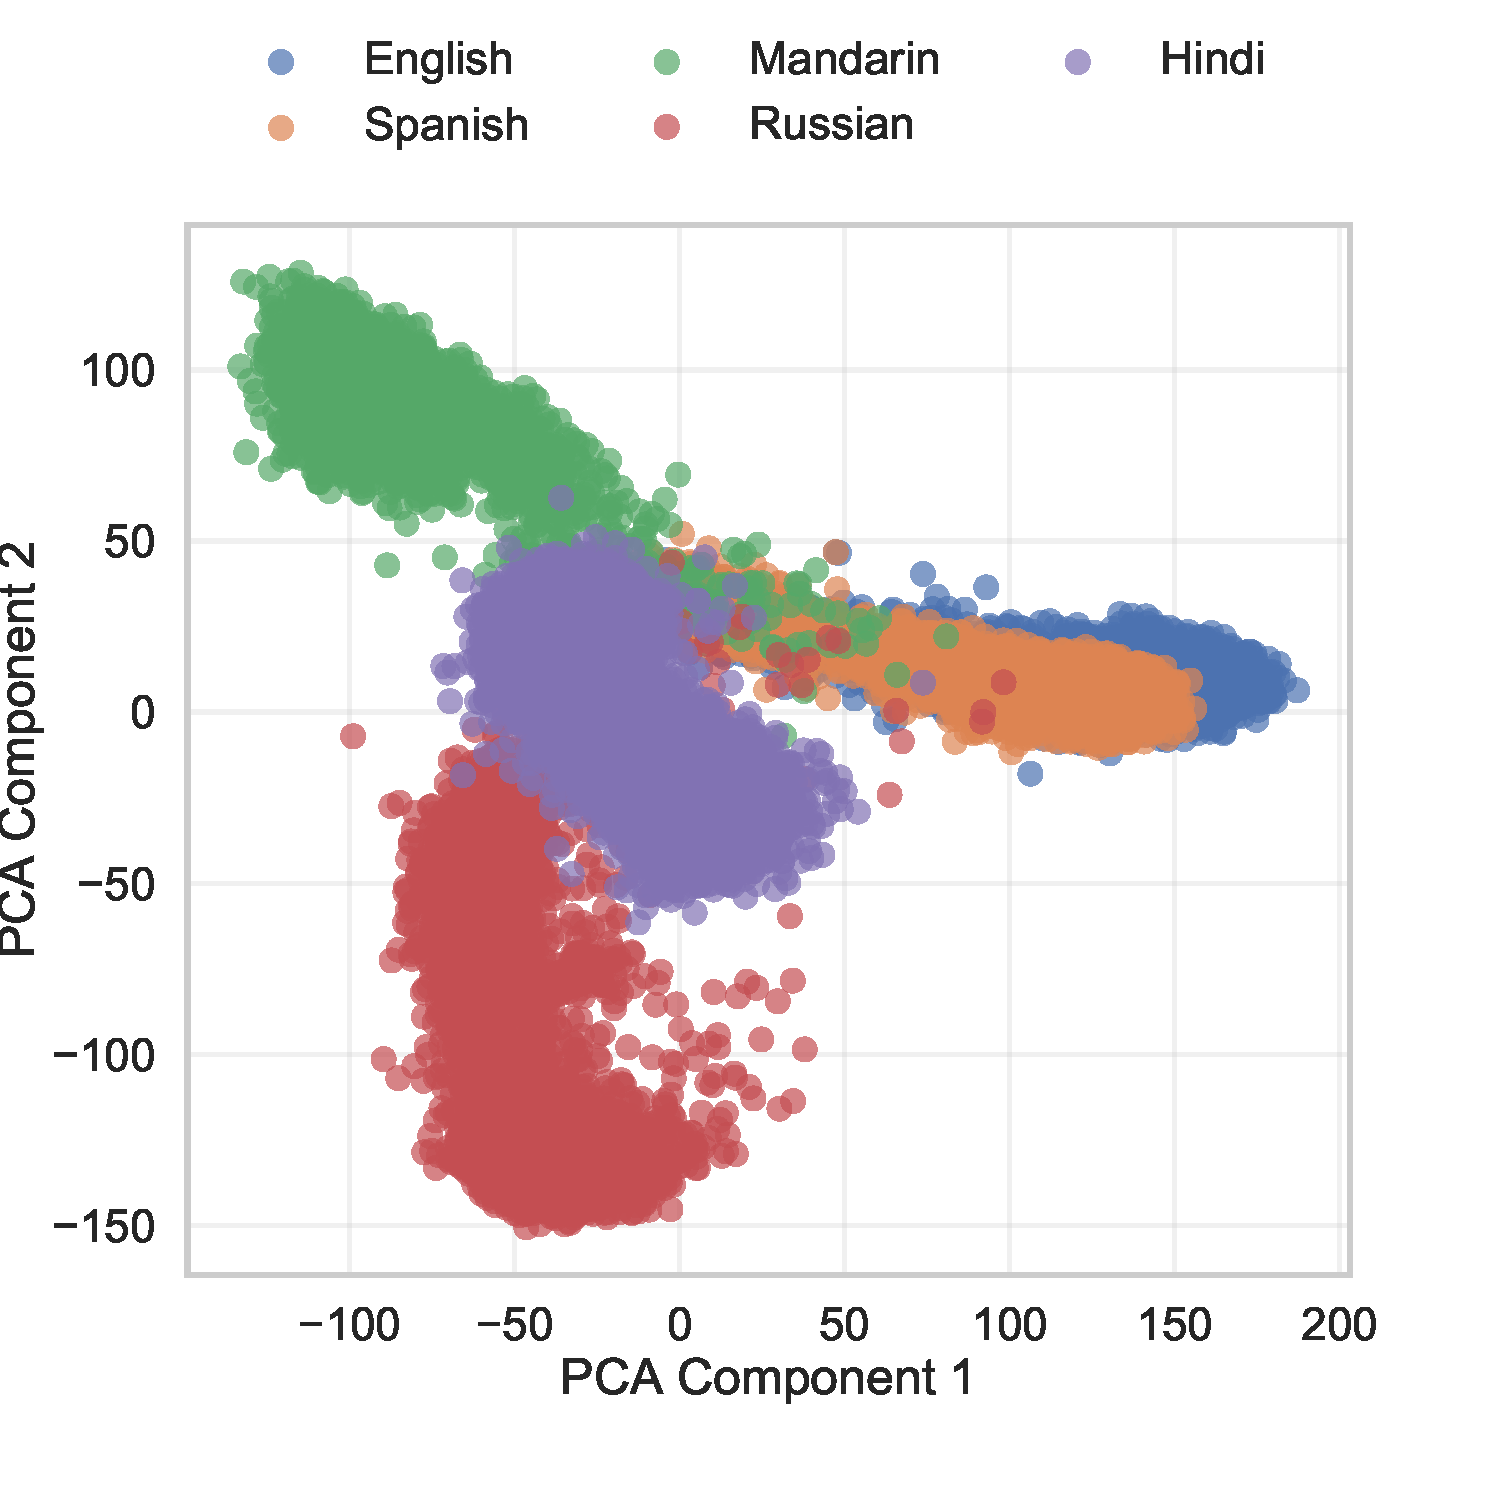
\includegraphics[width=1\linewidth]{images/language_map/multi/qwen/layer_28.pdf}
    \caption{Qwen}
    \label{fig:qwen_lang_map}
  \end{subfigure}
  \hfill
  \begin{subfigure}[b]{0.48\linewidth}
    \centering
    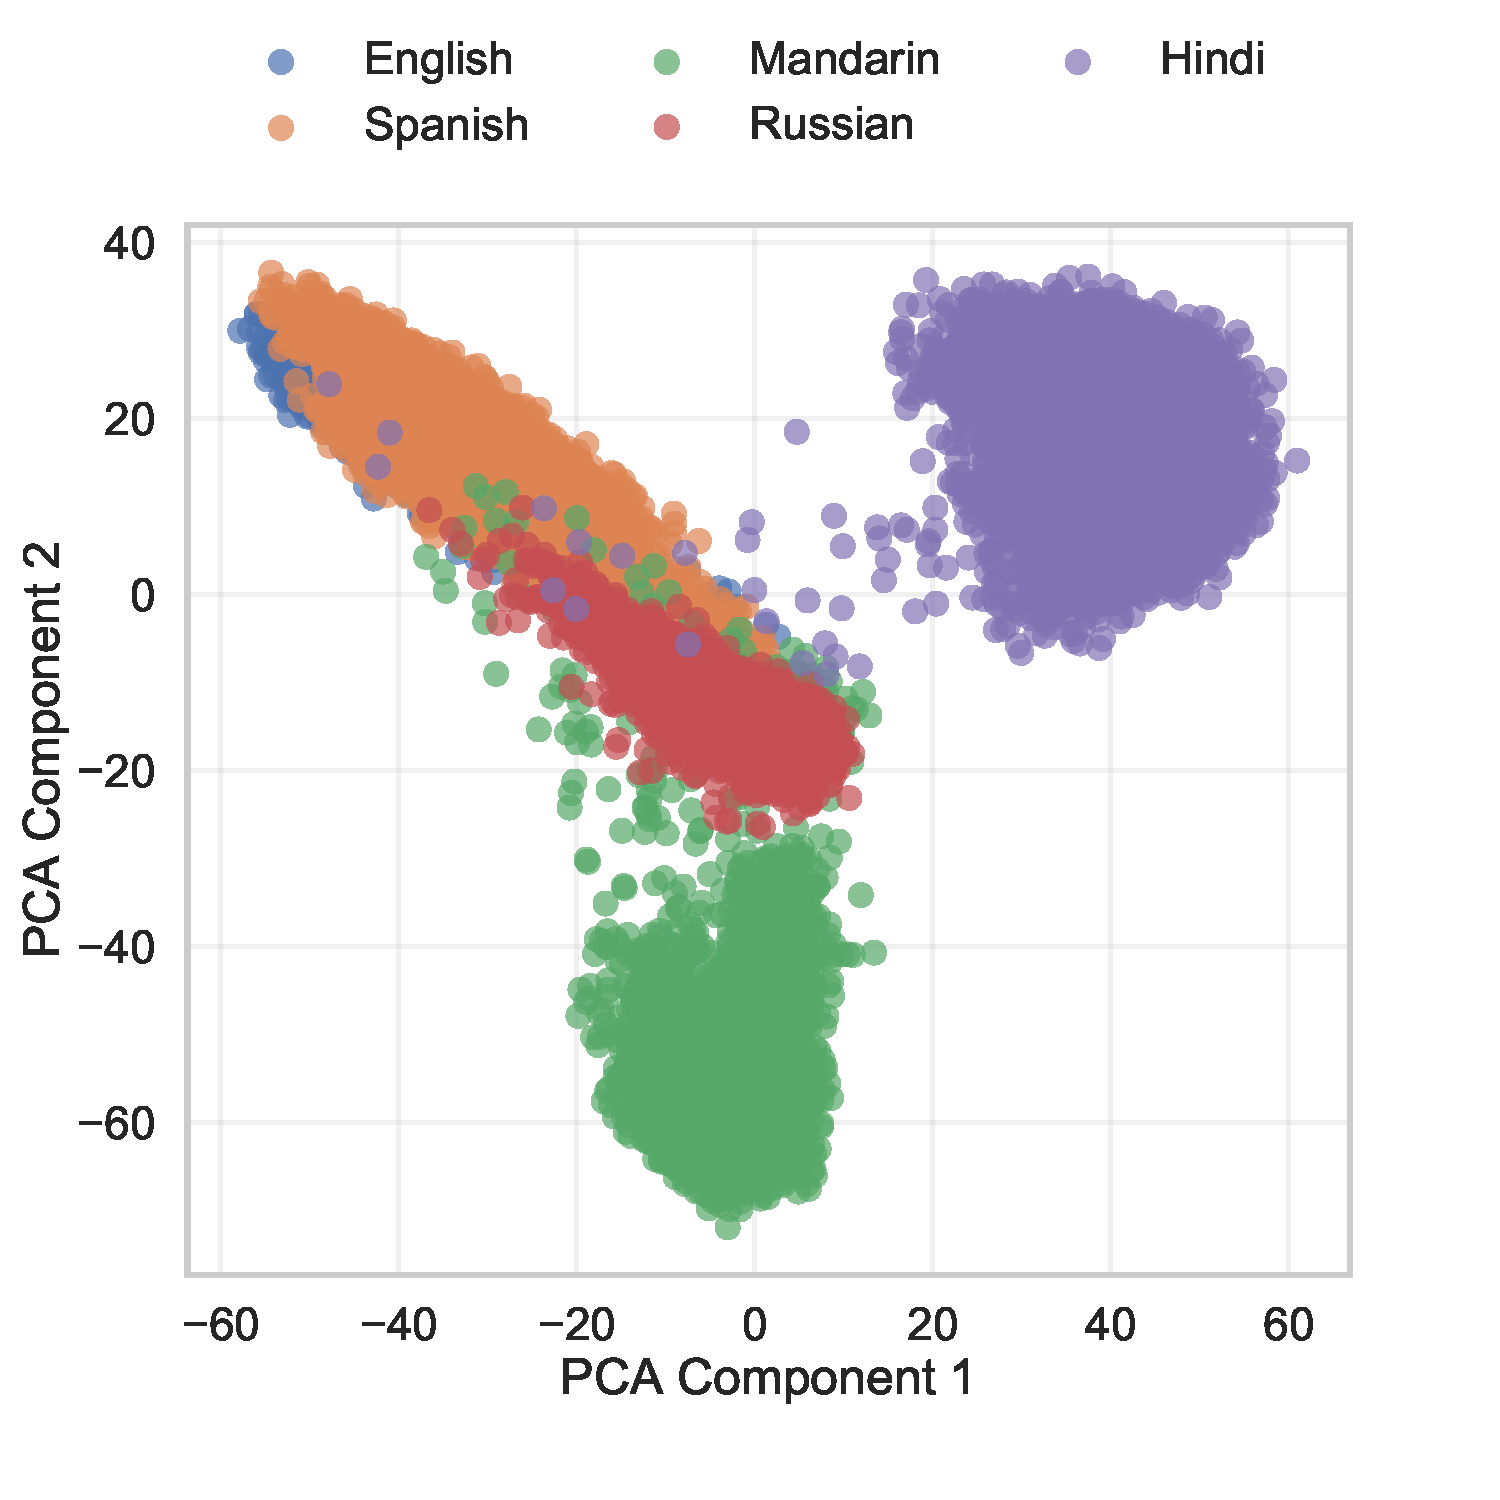
\includegraphics[width=1\linewidth]{images/language_map/multi/llama/layer_16.pdf}
    \caption{Llama}
    \label{fig:llama_lang_map}
  \end{subfigure}
  \caption{Final layer language map}
\end{figure*}

\begin{figure*}[ht]
  \centering
  \begin{subfigure}[t]{0.24\linewidth}
    \centering
    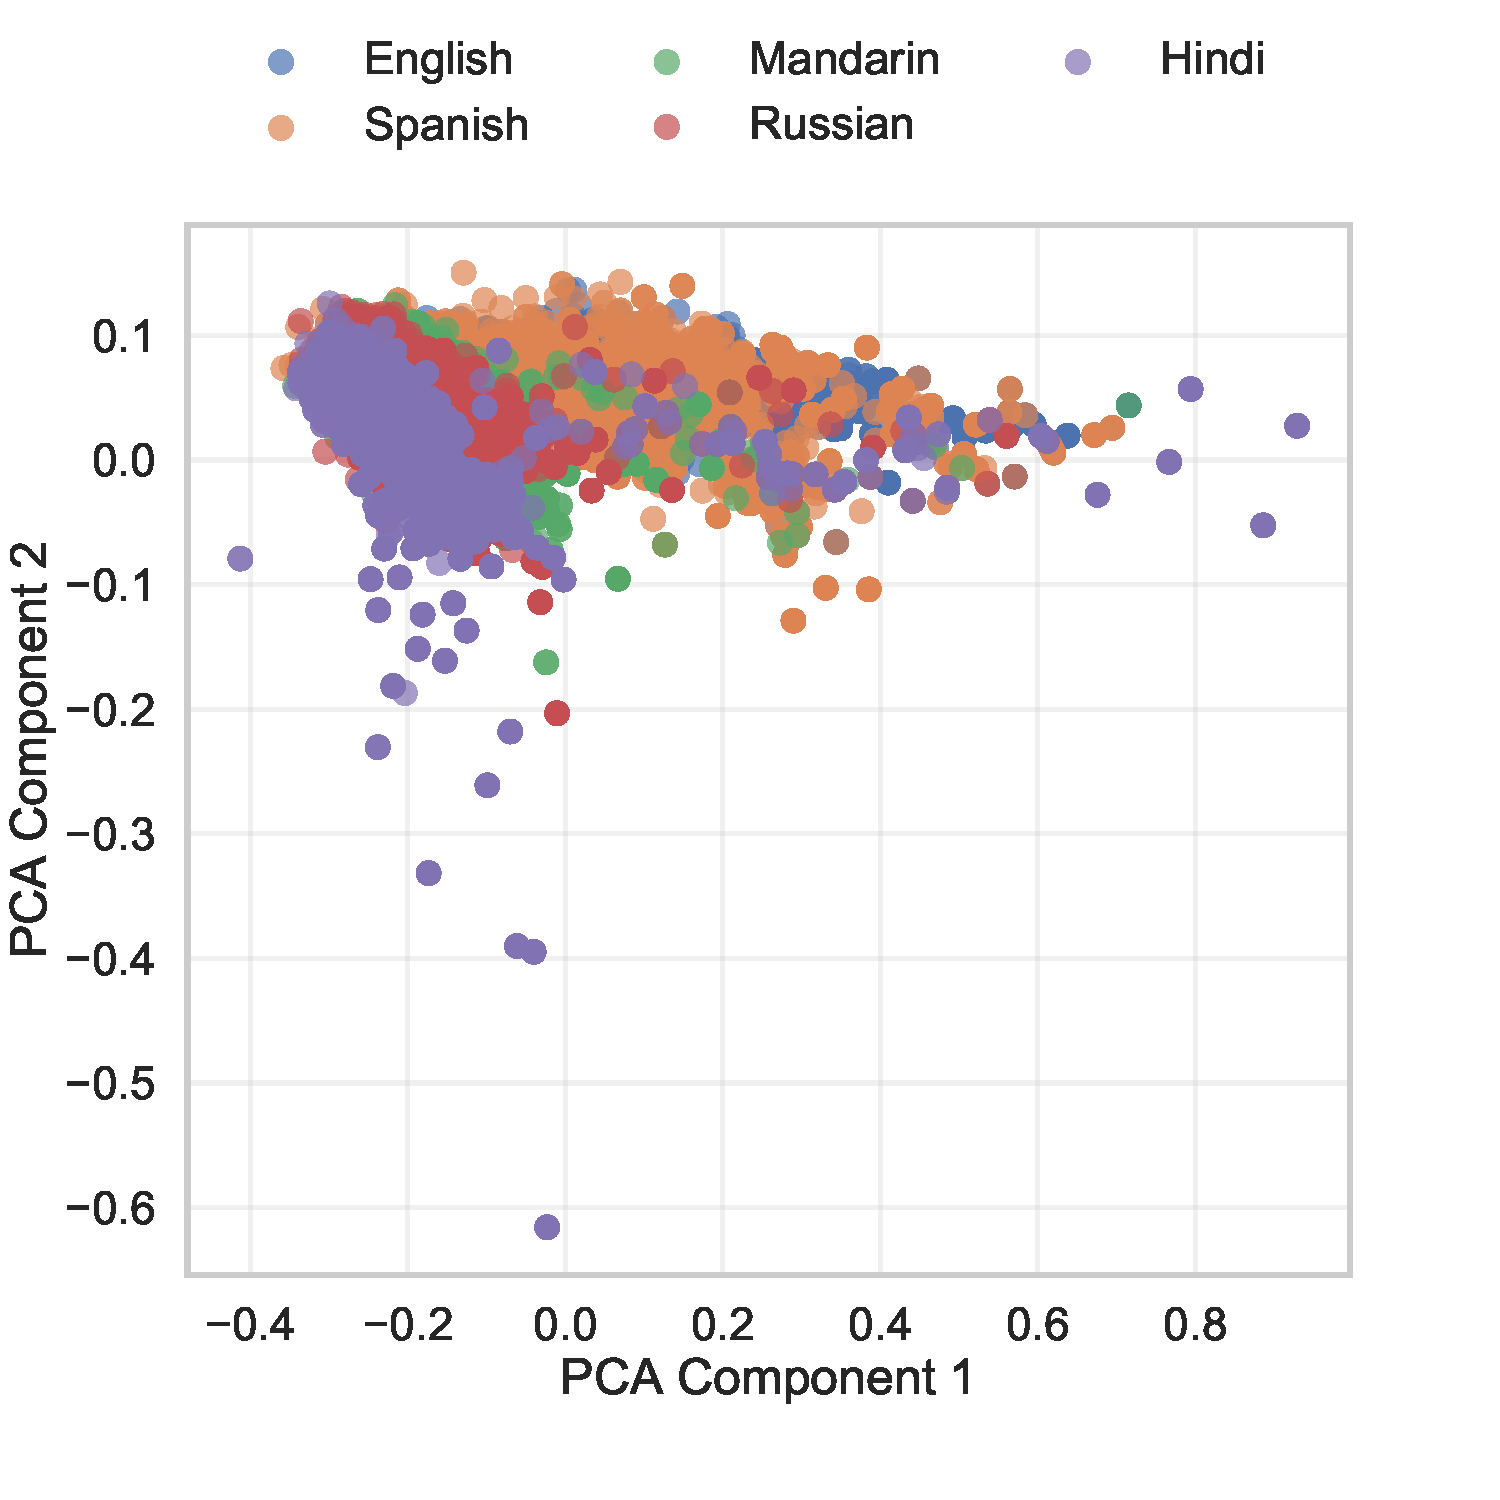
\includegraphics[width=1\linewidth]{images/language_map/multi/llama/layer_0.pdf}
    \caption{First layer}
    \label{fig:llama_lang_map_first}
  \end{subfigure}
  \hfill
  \begin{subfigure}[t]{0.24\linewidth}
    \centering
    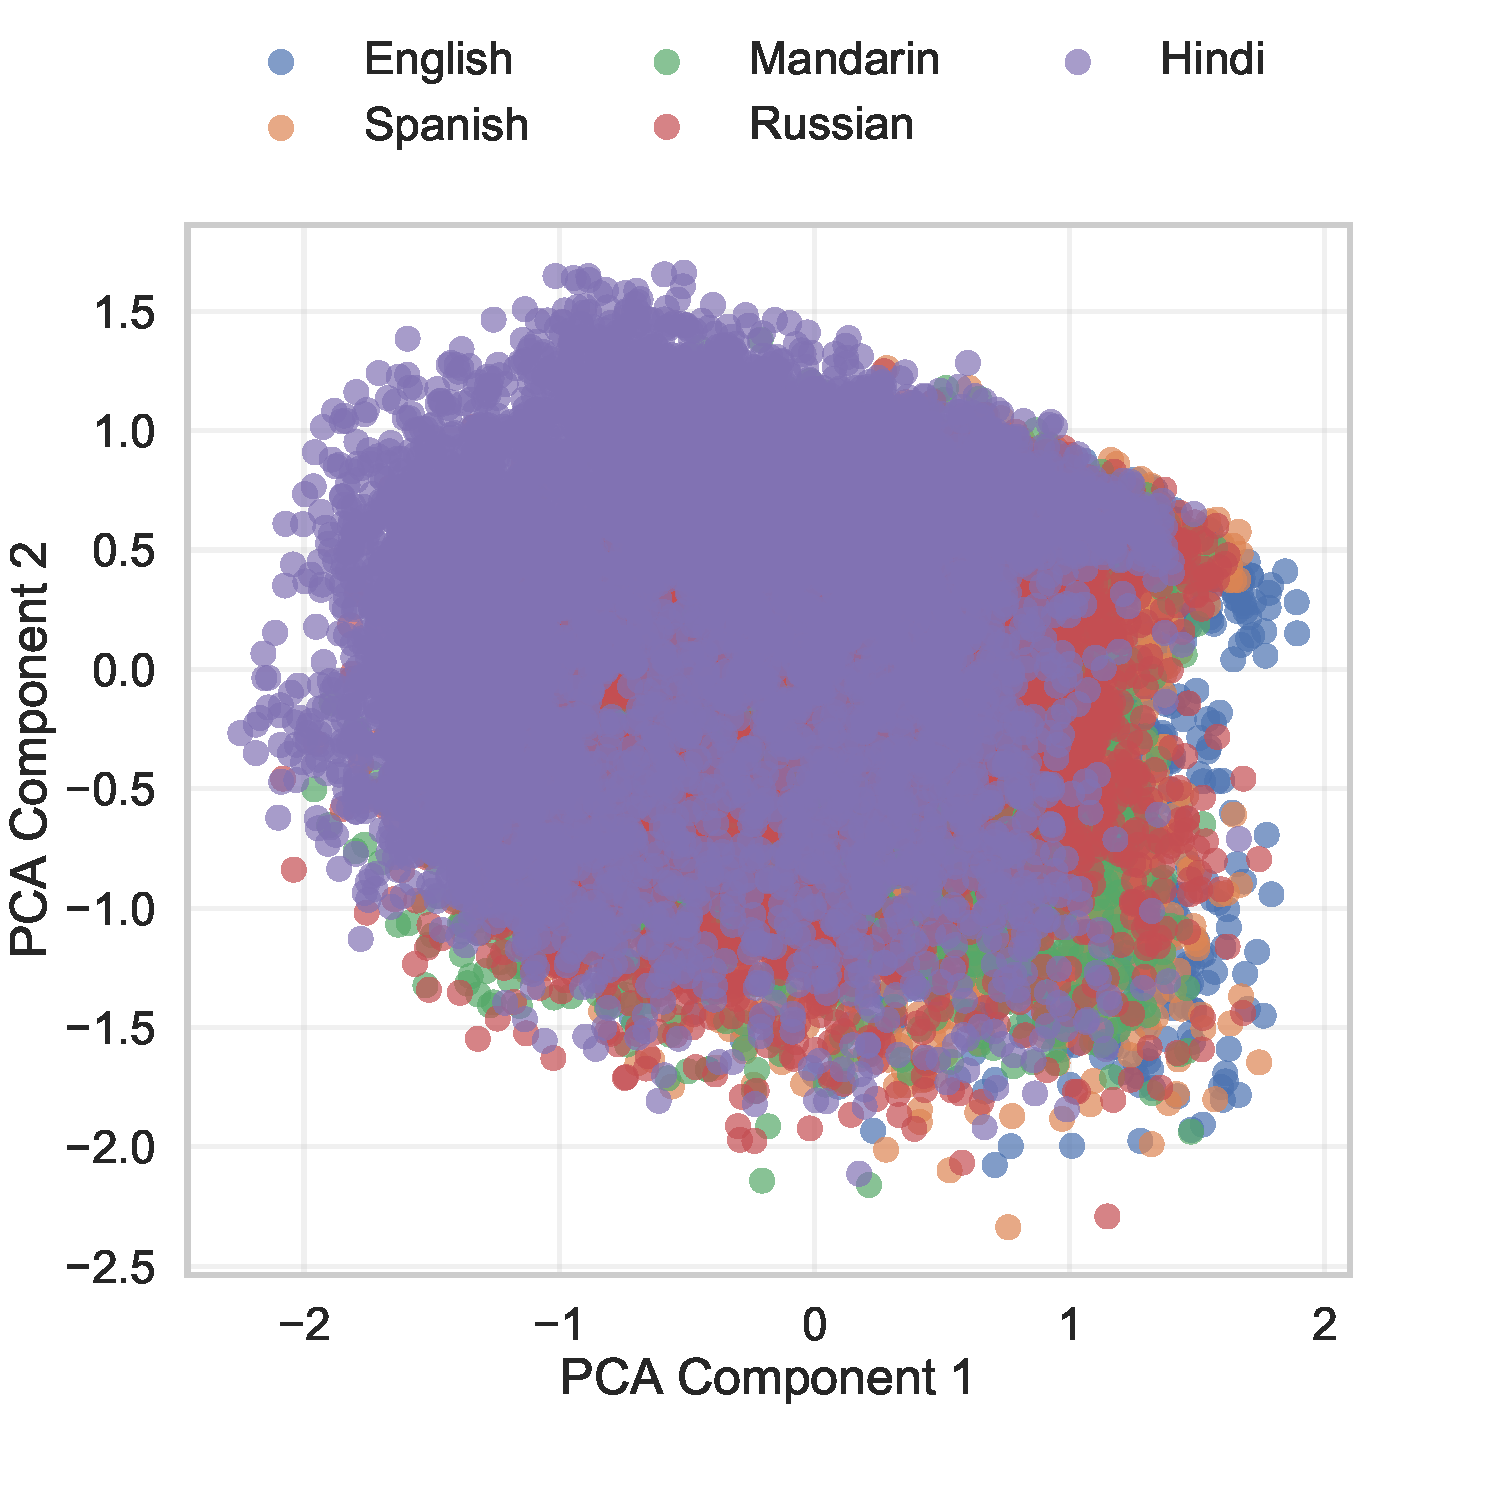
\includegraphics[width=1\linewidth]{images/language_map/multi/llama/layer_7.pdf}
    \caption{Mid layer}
    \label{fig:llama_lang_map_mid}
  \end{subfigure}
  \hfill
  \begin{subfigure}[t]{0.48\linewidth}
    \centering
    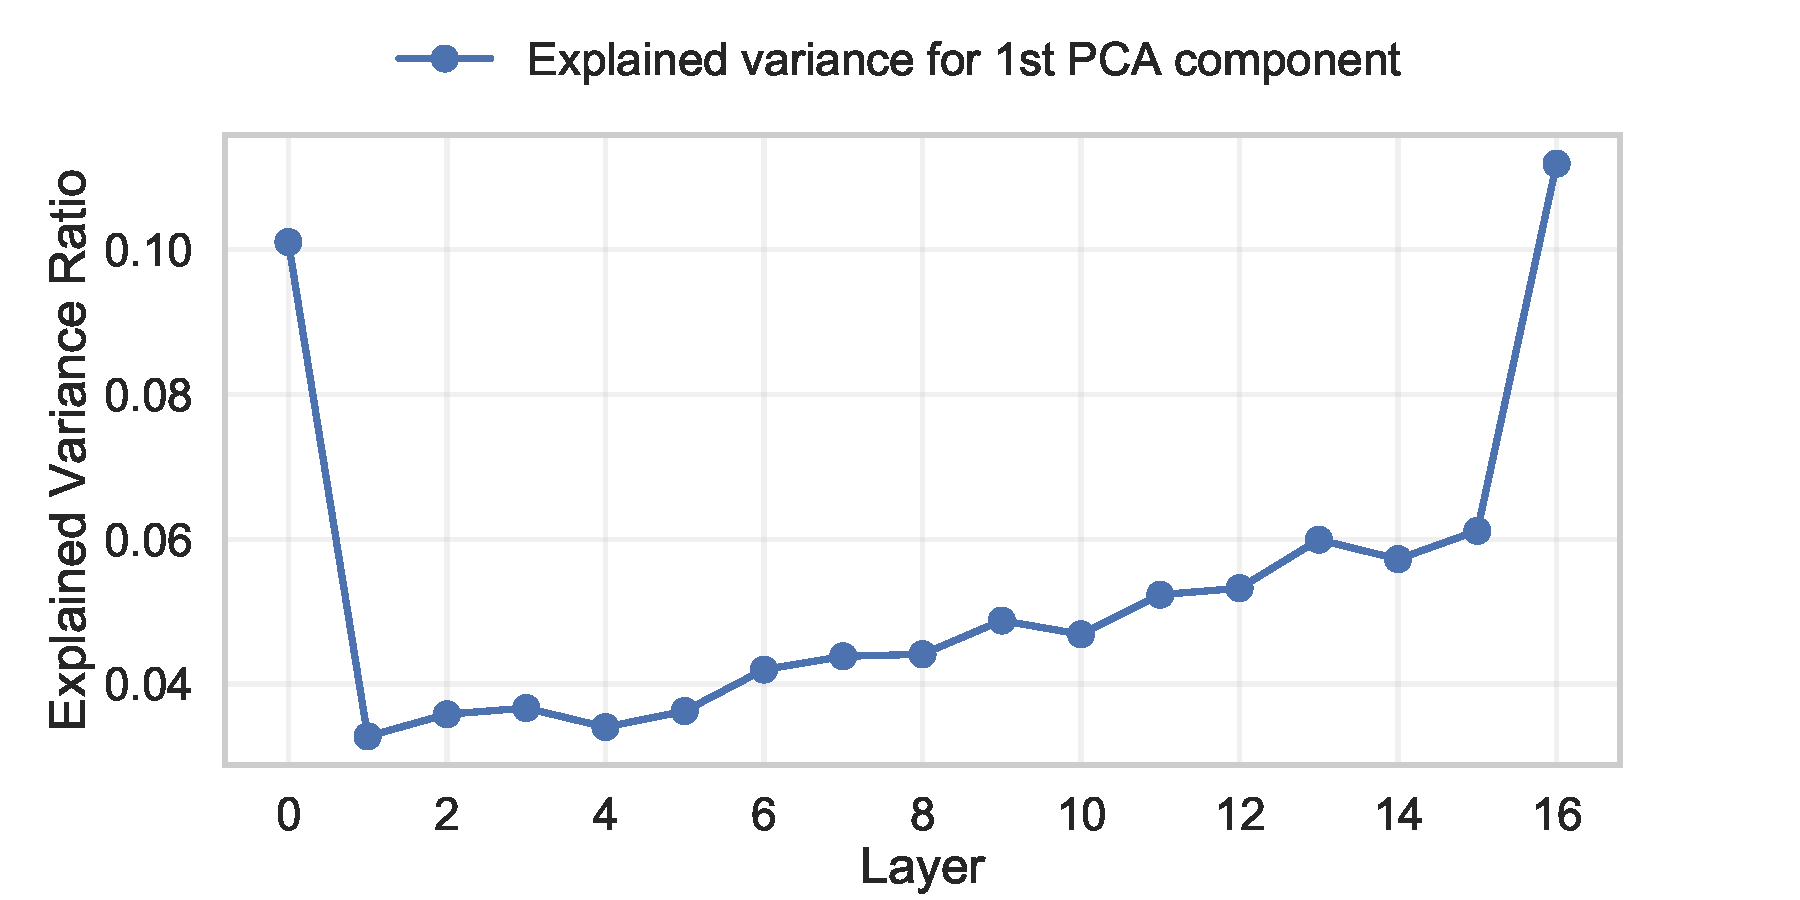
\includegraphics[width=1\linewidth]{images/language_map/multi/llama/explained_variance.pdf}
    \caption{Explained variance}
    \label{fig:llama_explained_variance}
  \end{subfigure}
  \caption{Llama layer-wise language maps and explained variance}
\end{figure*}

\begin{figure*}[ht]
  \centering
  \begin{subfigure}[t]{0.24\linewidth}
    \centering
    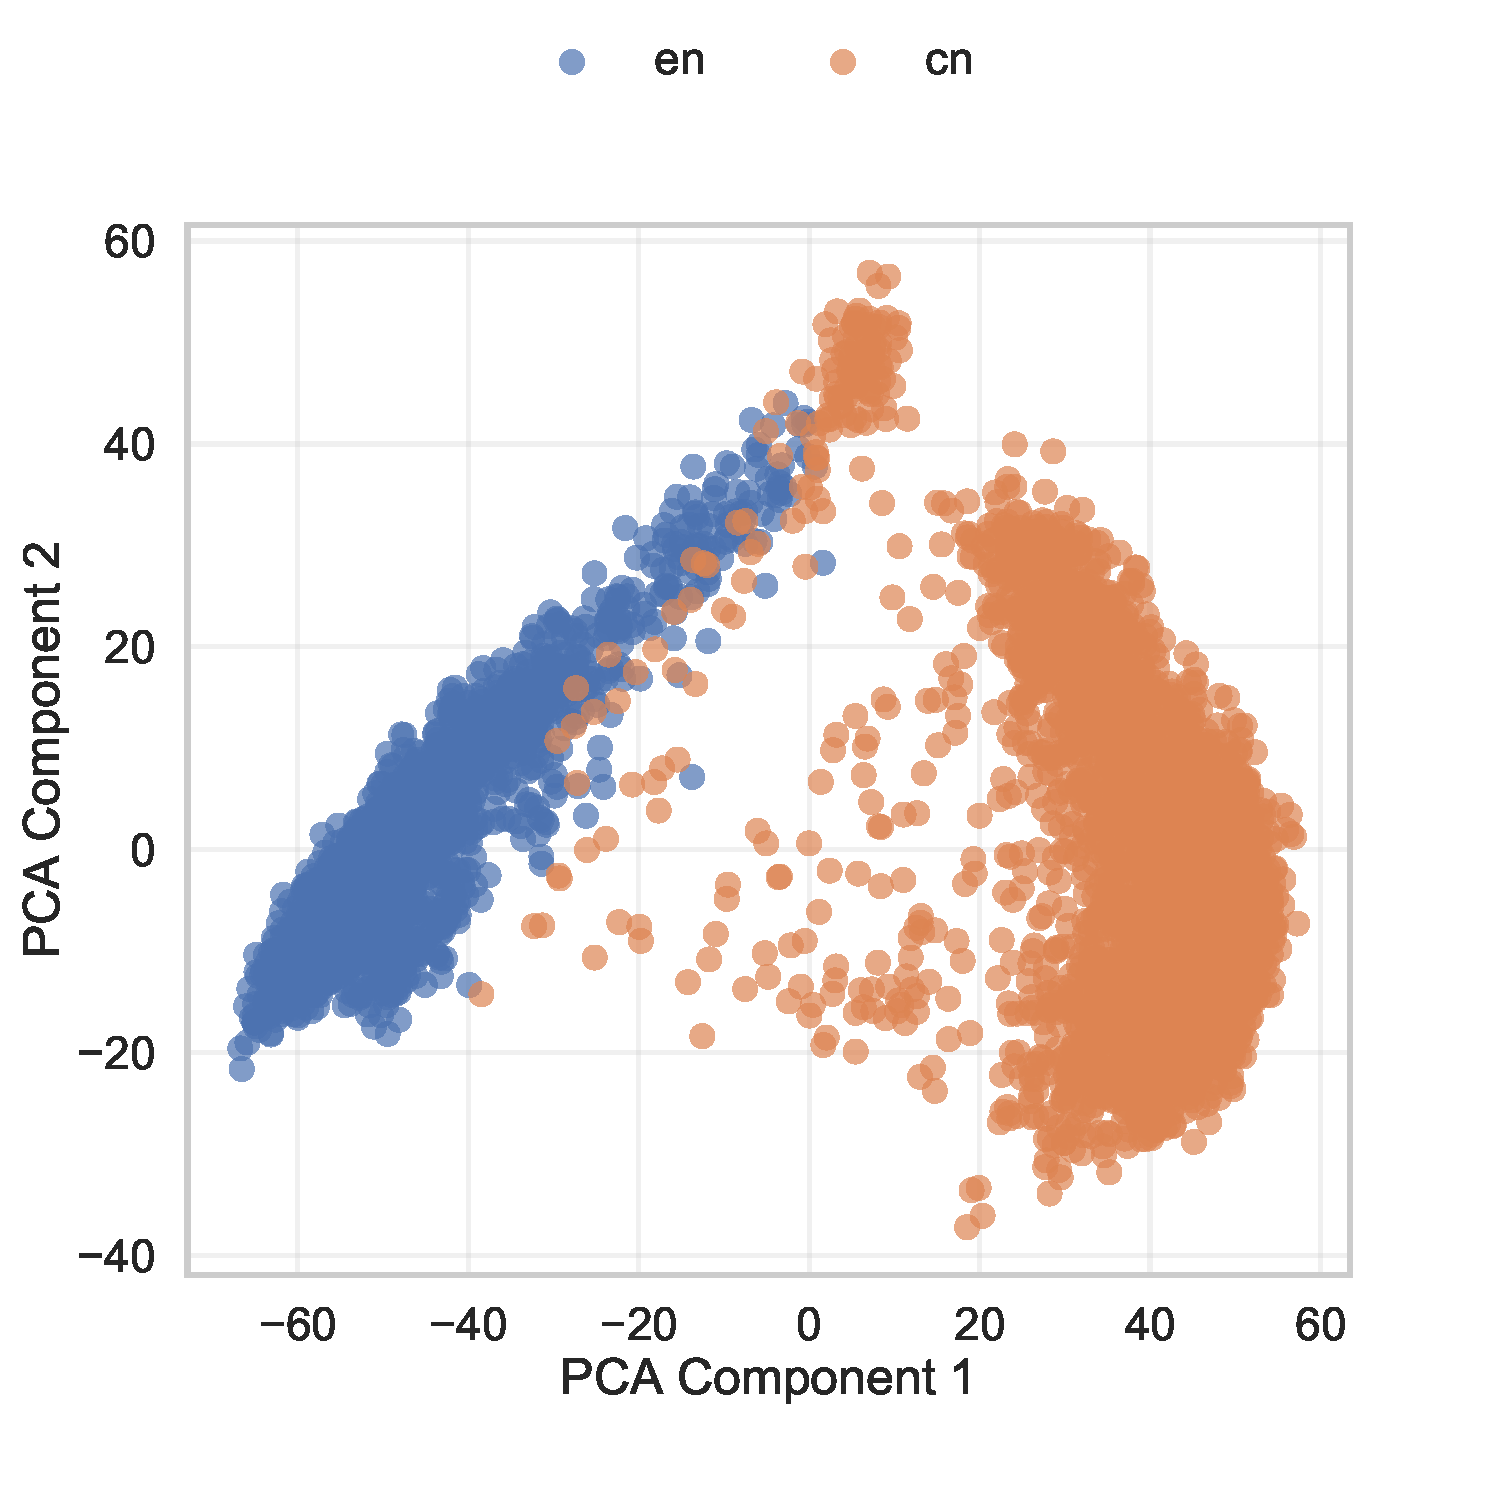
\includegraphics[width=1\linewidth]{images/language_map/en_cn/llama/layer_16.pdf}
    \caption{English - Chinese}
    \label{fig:llama_lang_map_en_cn}
  \end{subfigure}
  \hfill
  \begin{subfigure}[t]{0.24\linewidth}
    \centering
    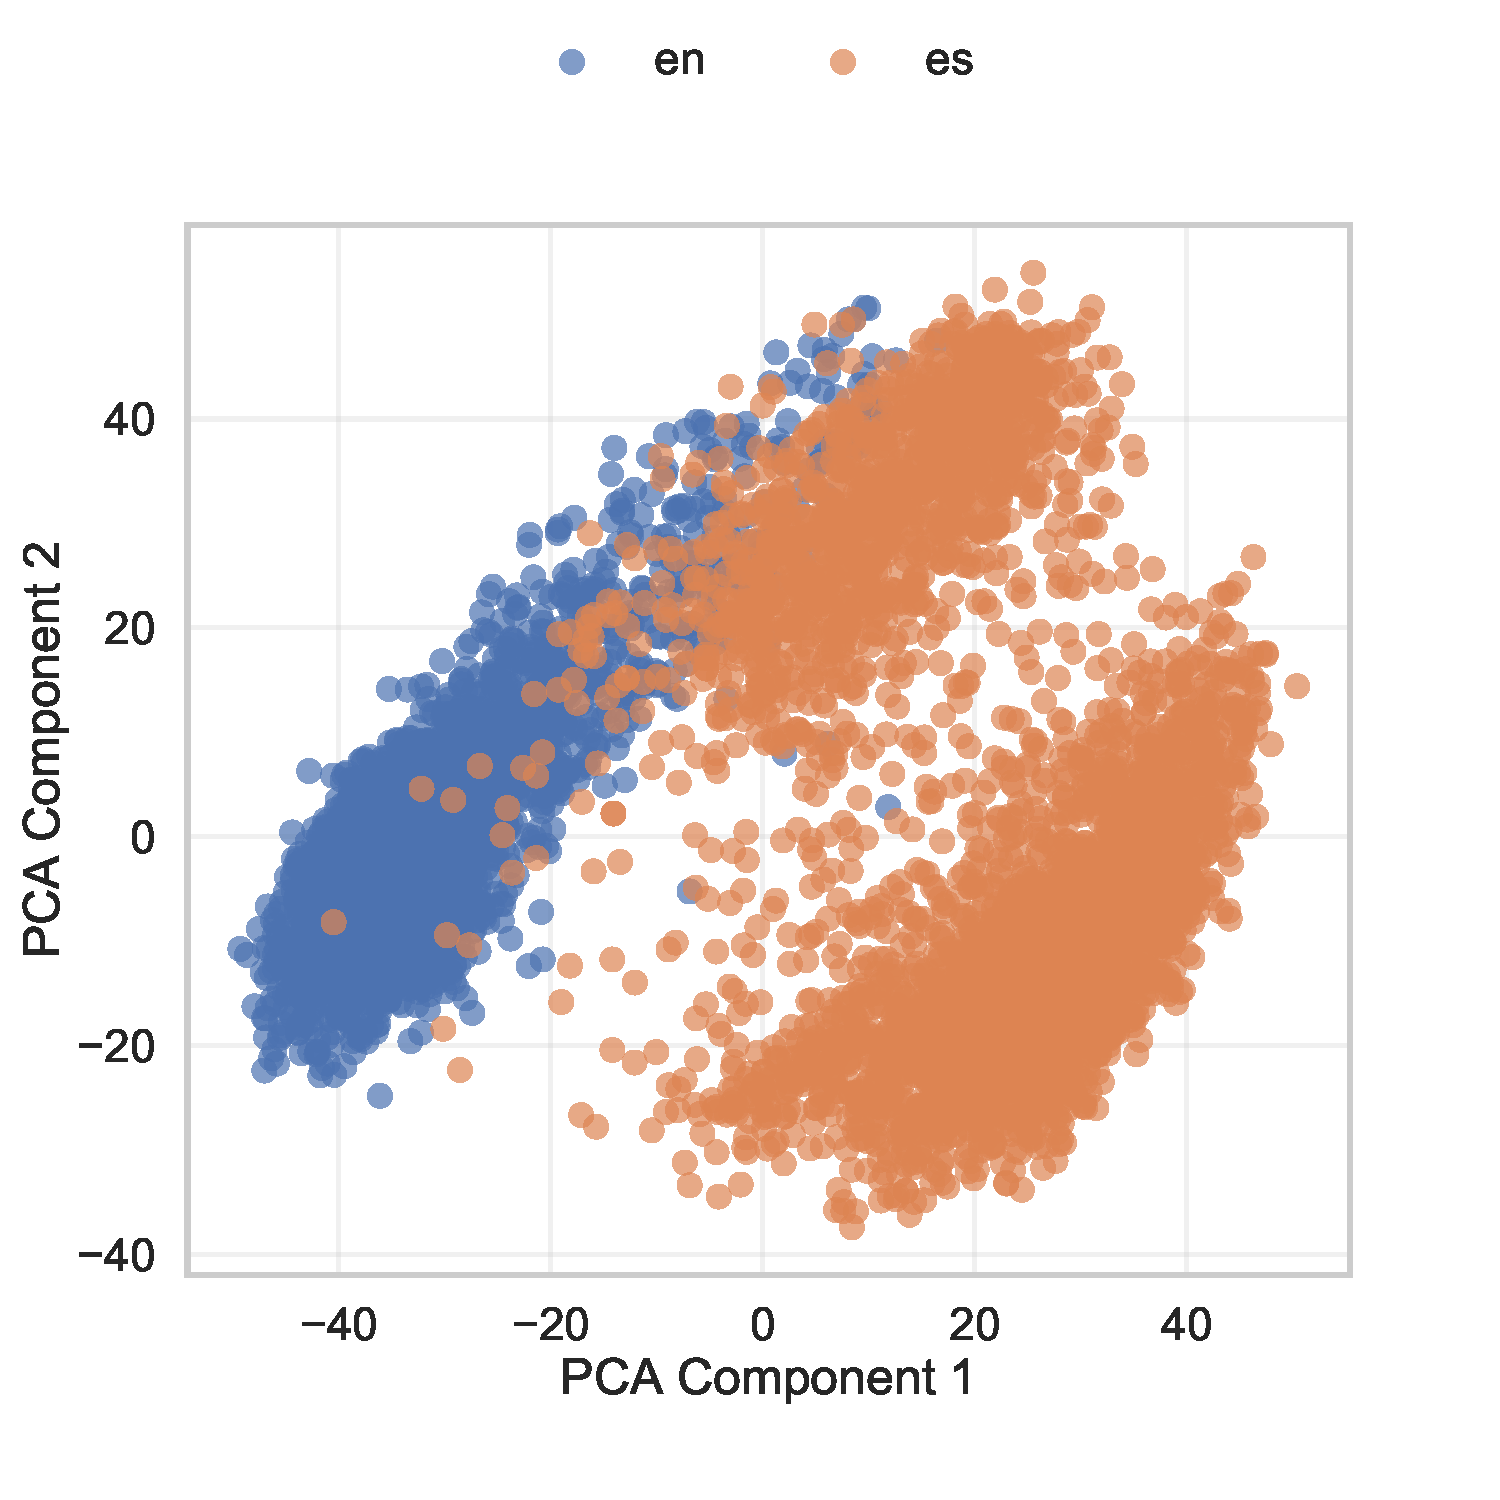
\includegraphics[width=1\linewidth]{images/language_map/en_es/llama/layer_16.pdf}
    \caption{English - Spanish}
    \label{fig:llama_lang_map_en_es}
  \end{subfigure}
  \hfill
  \begin{subfigure}[t]{0.24\linewidth}
    \centering
    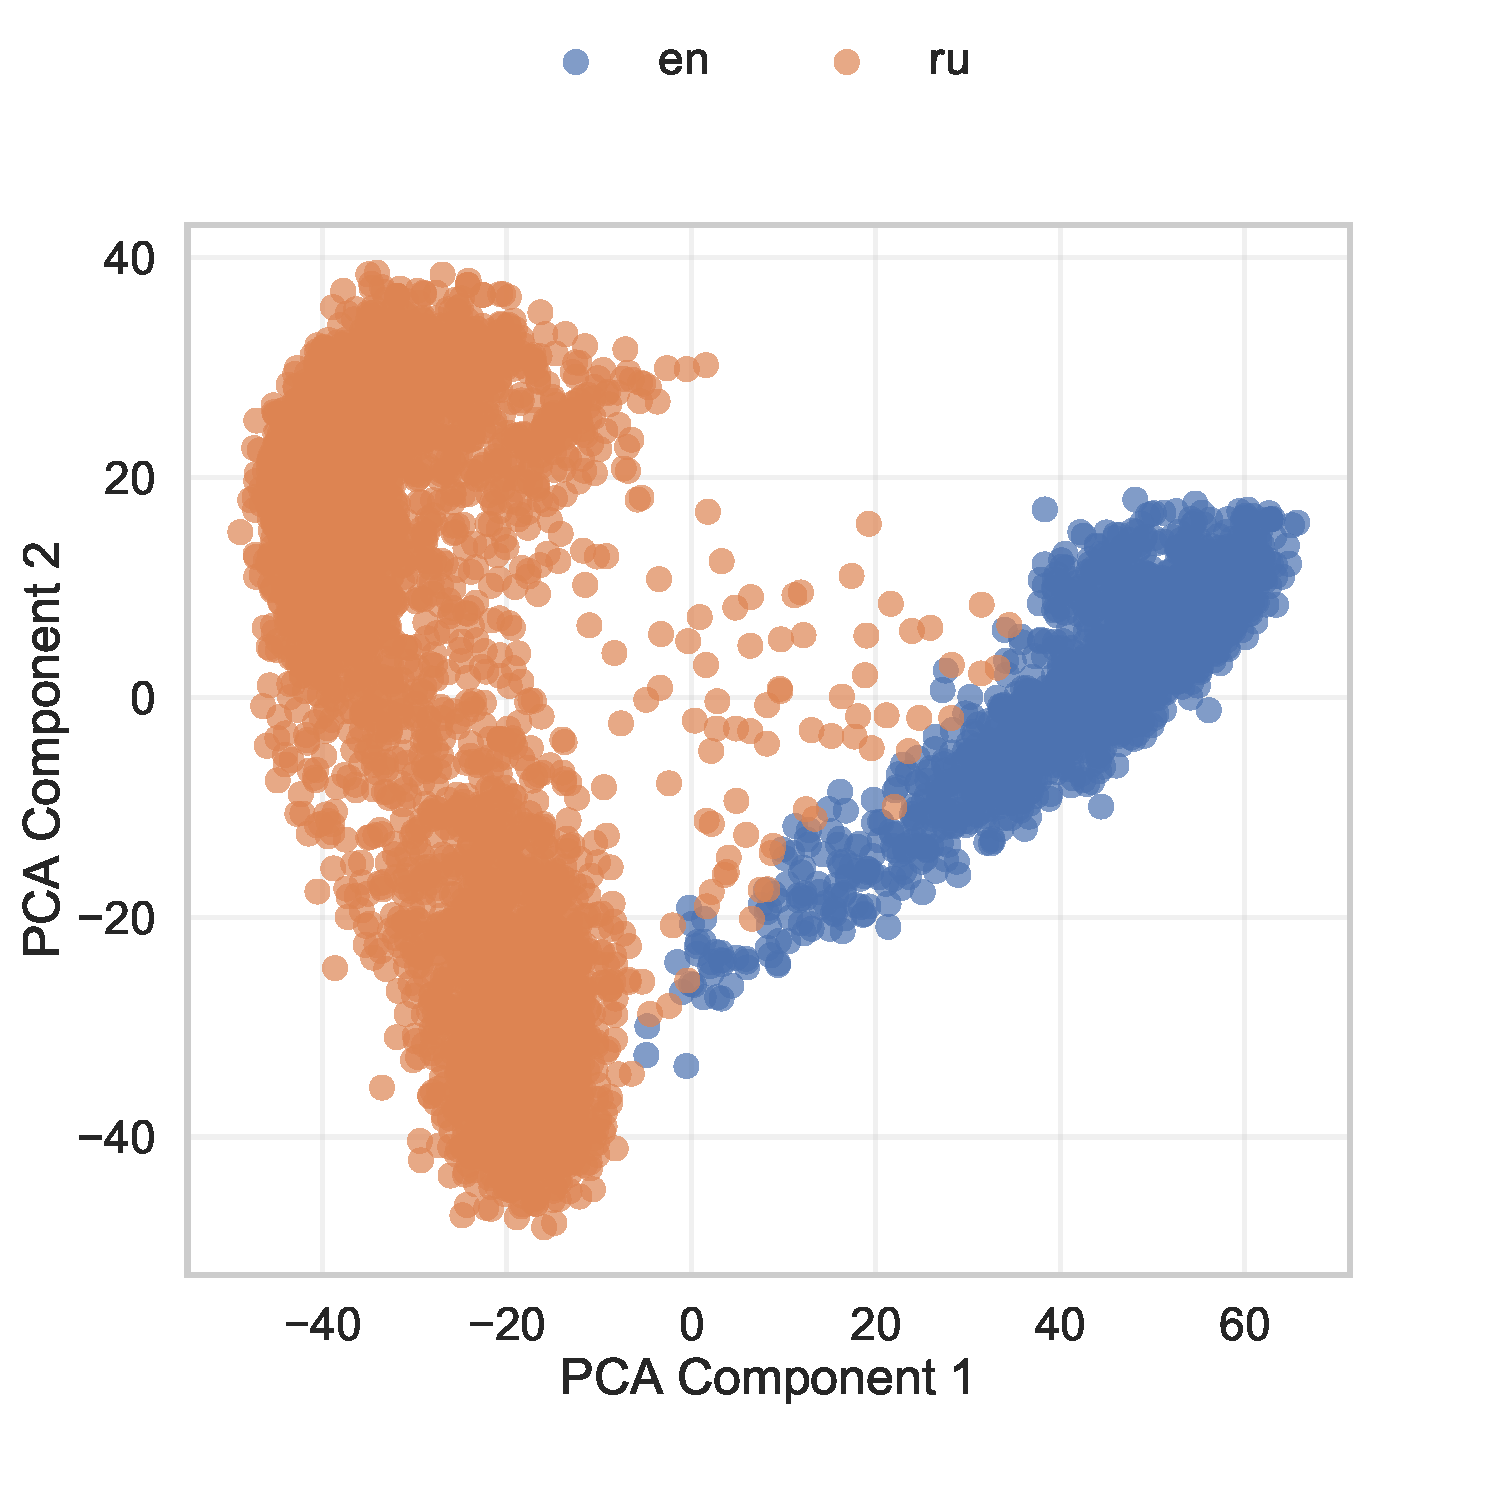
\includegraphics[width=1\linewidth]{images/language_map/en_ru/llama/layer_16.pdf}
    \caption{English - Russian}
    \label{fig:llama_lang_map_en_ru}
  \end{subfigure}
  \hfill
  \begin{subfigure}[t]{0.24\linewidth}
    \centering
    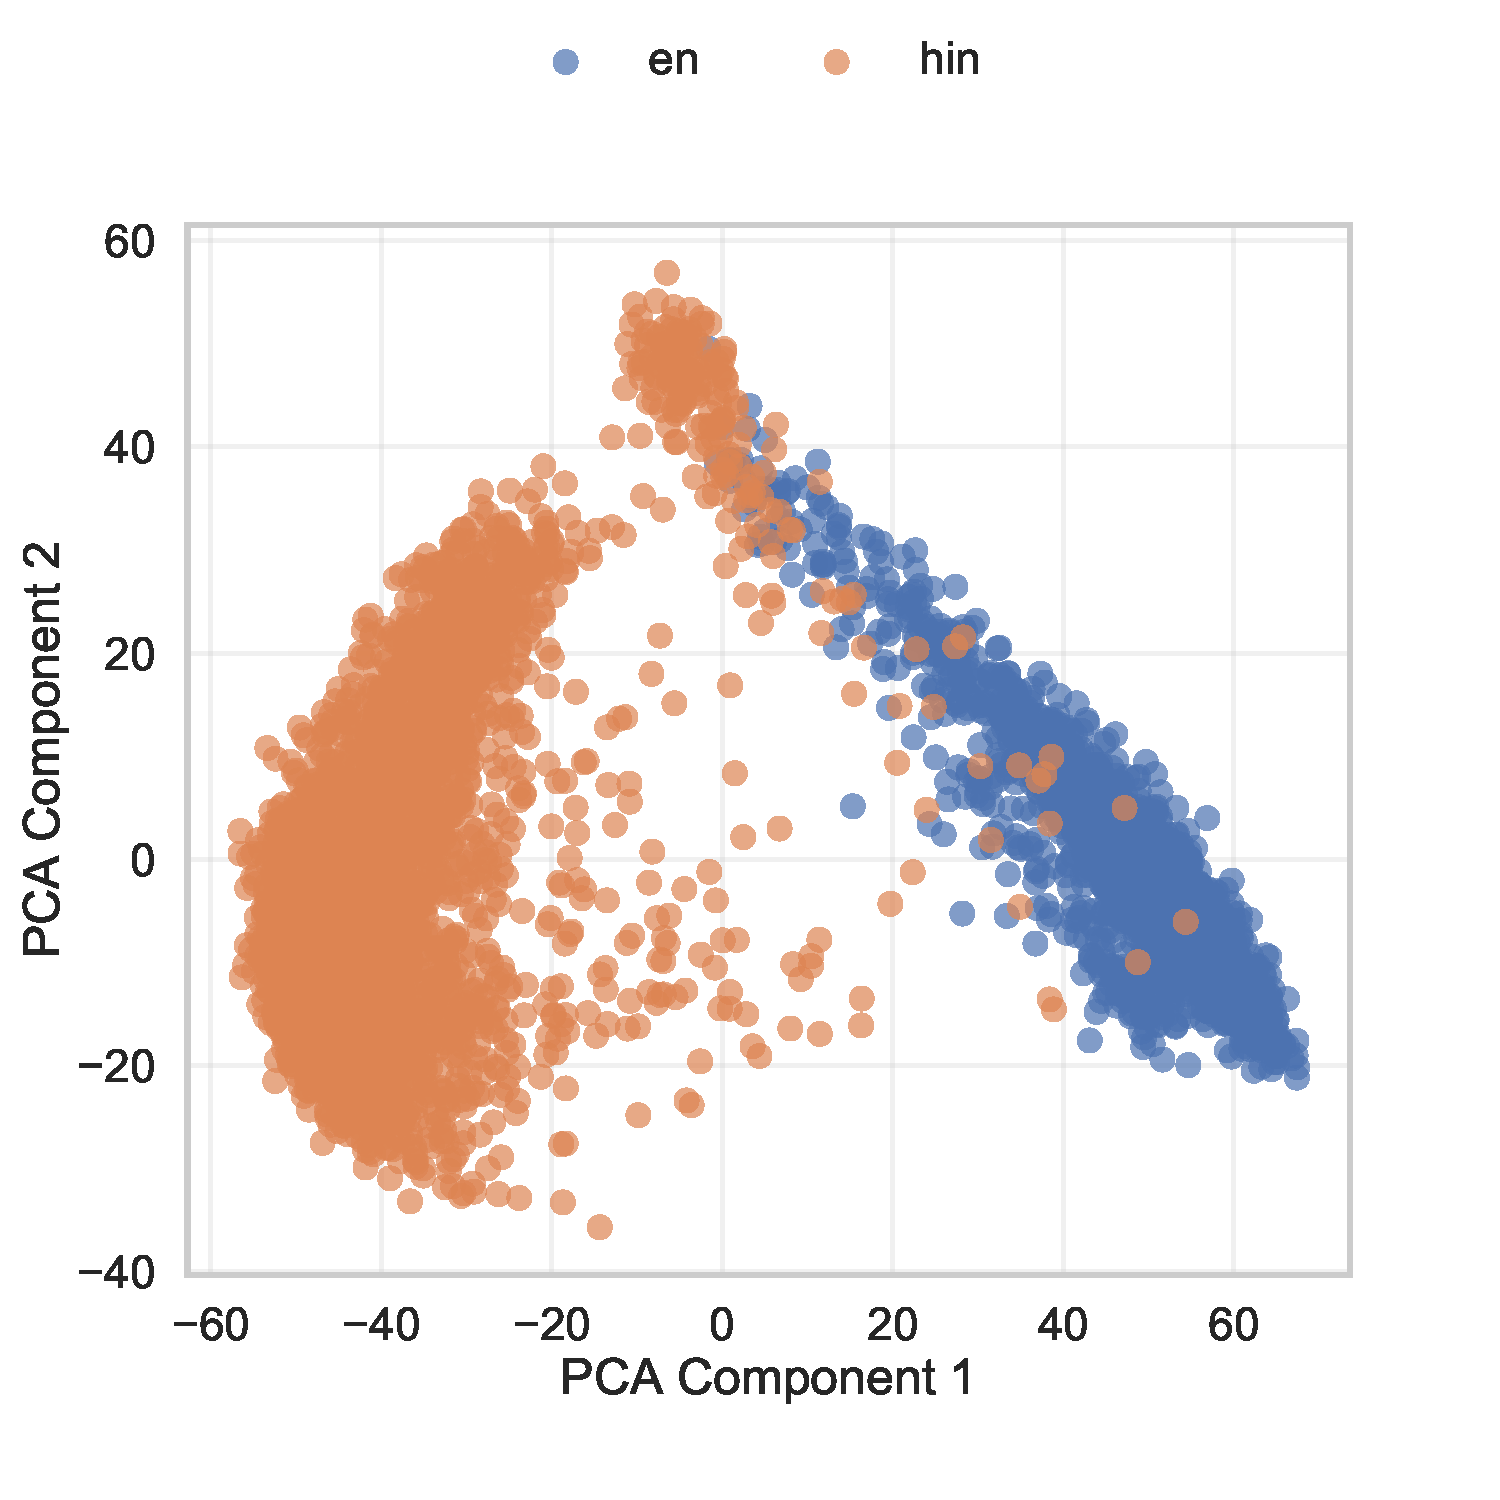
\includegraphics[width=1\linewidth]{images/language_map/en_hin/llama/layer_16.pdf}
    \caption{English - Hindi}
    \label{fig:llama_lang_map_en_hin}
  \end{subfigure}
  \caption{Llama final layer language maps for each language pair}
\end{figure*}

\subsection{Language direction identification}

\paragraph{Experimental setup.} Dataset: Flores Plus \cite{scaling-2024} with 50 parallel samples (English, Spanish, Russian, Chinese, Hindi) for PCA fitting and 100 for validation. Models: Qwen2.5-1.5B ~\cite{qwen2025qwen25technicalreport} and Llama-3.2-1B ~\cite{grattafiori2024llama3herdmodels}.

\paragraph{Language maps reveal emergent clustering.} Figure~\ref{fig:qwen_lang_map} and~\ref{fig:llama_lang_map} show final-layer embeddings projected onto the first two PCs.
Consistent with prior findings~\cite{conneau-etal-2020-emerging, wendler-etal-2024-llamas}, models organize identical content into tight, language-specific clusters with clear boundaries.
Languages within the Indo-European family (Spanish, Russian) cluster closer than typologically distant pairs (English--Chinese), suggesting PC1 captures coarse language distinction while PC2 encodes finer linguistic properties.

Figures ~\ref{fig:llama_lang_map_first} ~\ref{fig:llama_lang_map_mid} show layer-wise evolution:
clusters emerge loosely in early layers and sharpen dramatically in final layers.
Figure~\ref{fig:llama_explained_variance} reveals late-stage specialization for language identity.
Pairwise maps (Figures ~\ref{fig:llama_lang_map_en_cn}, ~\ref{fig:llama_lang_map_en_es}, ~\ref{fig:llama_lang_map_en_ru}, ~\ref{fig:llama_lang_map_en_hin}) confirm clean linear separability for all tested pairs.

\paragraph{Language prediction.} We train a logistic regression classifier on final-layer projections. Classifier trained only on the first principal component achieves near-perfect accuracy (0.96-1.00) across all language pairs and both models (Table~\ref{tab:clf}).
We observe decreased performance for the English-Spanish pair in both models, attributable to these languages being more closely related to each other.
\subsection{Language steering}

\paragraph{Next-token distribution evaluation.} We fit the steering module on Flores Plus with 200 parallel samples and test on 2,467 TED Talks \citep{banik2017tedtalks} samples with artificial code-switching.
Each sample is truncated to 20 words, split at the midpoint, and the second half is translated to the target language using Gemini 2.5 Flash via the OpenRouter API, producing texts that begin in English and switch mid-sentence.
Success is measured by comparing the next-token prediction distribution of the steered model against the English baseline via: KL divergence $\text{KL}(P_{\text{EN}} \| P_{\text{steered}})$, cosine similarity, and top-50 token overlap.

Table~\ref{tab:kl_cos_overlap} shows steering reduces KL divergence, increases cosine similarity and token overlap across all models and language pairs with a notable inefficiency on English-Hindi language pair.
The method shifts predictions from Spanish tokens (muy, bastante, tan) to their English equivalents (very, quite, so) while preserving semantic coherence (Table~\ref{tab:token_sample}).
We hypothesize that model-specific tokenization and training data balance play a key role. The Qwen model processed much more English and Chinese data, leading to more granular tokenization and better internal generalization for that pair.
At the same time, Hindi representation in the training corpus is usually much poorer.

\begin{table}[h]
  \centering
  \small
  \begin{tabular}{l l l}
    \hline
    Language pair & Qwen & Llama \\
    \hline
    English - Chinese & 10.15 / 0.02 / 3.69\% $\rightarrow$   & 9.05 / 0.05 / 4.47\% $\rightarrow$  \\
    & 4.52 / 0.22 / 26.46\% & 4.77 / 0.21 / 24.31\% \\
    English - Spanish & 7.25 / 0.12 / 11.41\% $\rightarrow$ & 6.52 / 0.12 / 11.45\% $\rightarrow$  \\
    & 4.90 / 0.18s / 20.23\% & 3.48 / 0.29 / 30.74\% \\
    English - Russian & 8.70 / 0.09 / 7.41\% $\rightarrow$  & 7.77 / 0.10 / 7.49\% $\rightarrow$  \\
    &5.40 / 0.23 / 25.45\% & 3.49 / 0.31 / 31.96\% \\
    English - Hindi & 9.60 / 0.04 / 11.23\% $\rightarrow$  & 8.06 / 0.06 / 6.54\% $\rightarrow$  \\
    &7.02 / 0.07 / 11.68\% & 6.13 / 0.16 / 25.88\% \\
    \hline
  \end{tabular}
  \caption{KL divergence / Cosine similarity / Top-50 token overlap (no steering $\rightarrow$ steering)}
  \label{tab:kl_cos_overlap}
\end{table}

\begin{table}[h]
  \centering
  \small
  \begin{tabular}{l c c c}
    \hline
    & & \multicolumn{2}{c}{Steered} \\
    \cmidrule(lr){3-4}
    Language pair & Unsteered & KL-opt. & CSI-opt. \\
    \hline
    English - Chinese  & 0.64 & 0.03 & 0.03 \\
    English - Spanish  & 0.62 & 0.23 & 0.11 \\
    English - Russian  & 0.59 & 0.02 & 0.01 \\
    English - Hindi    & 0.81 & 0.04 & 0.01 \\
    \hline
  \end{tabular}
  \caption{Code-Switching Index (CSI, $\downarrow$) of generated text (Llama-3.2-1B, $n=500$, code-switched input). English-only baseline: CSI~$= 0.02$. }
  \label{tab:gen_results}
\end{table}

\begin{table}
  \centering
  \small
  \begin{tabular}{l c c c}
    \hline
    & Qwen & \multicolumn{2}{c}{Llama} \\
    \cmidrule(lr){2-2} \cmidrule(lr){3-4}
    Language pair & KL-opt. & KL-opt. & CSI-opt. \\
    \hline
    English - Chinese & $-3.2$ & $-5.0$ & $-5.0$ \\
    English - Spanish & $-2.8$ & $-3.7$ & $-5.0$ \\
    English - Russian & $-2.2$ & $-3.5$ & $-4.0$ \\
    English - Hindi   & $+5.0$ & $-3.6$ & $-5.0$ \\
    \hline
  \end{tabular}
  \caption{Best steering strength coefficients. KL-optimized: from the distributional grid search; CSI-optimized: from the generation grid search.}
  \label{tab:steering_coeff}
\end{table}

\paragraph{Generation-based evaluation.} To complement the distributional analysis above, we evaluate steering on actual text generation using Llama-3.2-1B.
For each of 500 TED Talks samples per language pair, we generate 100-token continuations in three conditions: (A)~English-only input without steering, (B)~code-switched input without steering, and (C)~code-switched input with steering.
We measure code-switching in the generated output with the \emph{Code-Switching Index} (CSI)~\cite{gamback-das-2016-comparing} and a FastText classifier~\citep{joulin-etal-2017-bag}.

We evaluate two sets of steering coefficients (Table~\ref{tab:steering_coeff}).
Notably, the optimal steering coefficient (Table~\ref{tab:steering_coeff}) for Qwen English-Hindi is positive ($+5.0$), indicating the biggest variance comes not from the language component, but from some other component of unexplored nature.
Coefficients are highly fragile: small changes in magnitude can shift the model from fluent code-switched output to degenerate repetition.
Table~\ref{tab:qualitative} shows representative examples.

Table~\ref{tab:gen_results} shows that steering substantially reduces code-switching in generated text. CSI-optimized coefficients tend toward higher magnitudes, which improves language control but increases degeneration risk (see Limitations).
